\documentclass[10pt,conference,compsocconf]{IEEEtran}

% !BIB program = biblio

\usepackage{url}
\usepackage{graphicx}
%\usepackage{amsmath}
\usepackage{caption}
\usepackage{subcaption}

\pagestyle{plain}

\begin{document}
\title{
  Semester Project: Road Segmentation\\
  \large Computational Intelligence Lab\\
}

\author{
  Nicolas K{\"u}chler, Octavio Mart{\'i}nez, Sabina Fischlin,\\
  group: \textit{TheRoadSegmenters},\\
  Department of Computer Science, ETH Zurich, Switzerland
}

\maketitle

\begin{abstract}
The road segmentation problem as given in the semester project description has the goal to label patches of 16x16 pixels as either \textit{road} or \textit{background}. In our solution we have trained two different models, one a \textit{UNet} and the other a modified  \textit{SqueezeNet}, and have post-processed the obtained predictions on the test images using  \textit{conditional random fields (CRF)}. The two models chosen each were able to identify different features of a road. For our final results we have output the average of the post-processed prediction probabilities from both models. By combining the two solutions, we were able to unite their respective strengths. The use of CRF as a post-processing mechanism has successfully been able to remove many false predictions, in particular when a background pixel was falsely labelled as a \textit{road}.  \\
In order to achieve more accurate results we have extended the given training data set with additional (self-labeled) images from \textit{Google Earth} and have also run all images from the training set through an augmentation process.\\
We also present a SqueezeNet architecture adapted to an image segmentation problem.
\end{abstract}

\section{Introduction}
With their results clearly dominating over other models, neural networks have become the state of the art for image segmentation problems. Our first approach to the road segmentation challenge was therefore to implement a UNet. The UNet model was first proposed in~\cite{RFB15a} for biomedical image segmentation and is now one of the most successful~\cite{IEEE1} models for image segmentation in general.

We have found however, in our earliest test runs using only the UNet model, that while it did well on certain image areas (e.g. green areas and highways), it would perform badly on others (e.g. parking lots, roads with varying texture). What if a model with an entirely different architecture was able to perform better on the areas that the UNet was missing? In other words, we aimed to complement the results of one model with the results of another.

While deeper networks usually yield much better results their performance is also quite low. SqueezeNet was created in an attempt to use smaller networks with higher performance which could produce just as strong results as deep networks~\cite{CoRR1}. With SqueezeNet being a simpler model it is also much easier to control what the network learns. SqueezeNets are typically used for multi-label classification problems. With small adjustments to its classical architecture we were able to adapt it to the needs for the binary segmentation problem at hand.

We have also found that especially the UNet would make many false predictions (i.e. labeling a patch as \textit{road} instead of \textit{background}) and merely averaging over the prediction probabilities of both models would not be able to eliminate this problem. \textit{Conditional random fields (CRF)} are used to create smoother results by maximizing the agreement on labels between similar pixels~\cite{NIPS2011_4296}. In other words, CRF have the ability to remove straying predictions.

In the next section we propose a combination of these techniques to improve the prediction precision.

\section{Models and Methods}
\subsection{Data Augmentation}
With the provided training data set only comprising 100 images, we opted to augment the data using the library \textit{Augmentor}~\cite{AugmeGL}. Although this would add another layer of non-determinism we decided to use online augmentation, i.e. re-augmenting the data at the beginning of every session, instead of augmenting the data only once. This has the advantage that the training data is as varying as possible. However, this meant that we did not have a fixed data set for the training of the models and therefore fixed the number of batches per epoch.

We have applied a combination of random basic transformations such as flips (horizontally and vertically), rotations (90$^{\circ}$, 180$^{\circ}$ and 270$^{\circ}$), random rotations by $\pm$ 25$^{\circ}$, shears and zooms. Additionally we have applied color transformations, especially as a counter measure against the issues arising from differences in brightness and colors of roads. In particular brightness, contrast, and PCA color augmentation as described in~\cite{NIPS2012_4824} have been performed.

\subsection{Training of the Models}
For the training of both models we used a square loss function. In order to evaluate the models we set aside 10-15 images (dependent on the data set used, see \textit{section~\ref{sec:dataset-extension}} for more information) from the training set to the validation set. These were selected according to their representation of different challenges with regards to predicting the presence of a road.

Our implementation uses \textit{tensorflow} and employs its \textit{Adam Optimizer}. We now describe the models and their architecture in detail.\\

\subsubsection{UNet}
A UNet consists of an encoder and a decoder --- much like a normal autoencoder. What sets it apart is its U-like architecture, with the encoder and decoder part consisting of several levels. Each level contains an encoder and a decoder block (except for the first layer which includes special input and output blocks). A speciality of the UNet architecture are the skip connections between the blocks of the same level (see left side of \textit{figure~\ref{fig:unet-arch}}). For our implementation of the UNet we have been inspired by its use in another Kaggle competition on satellite imagery feature detection, where its application was applied to a similar task~\cite{Dstl}.

The encoder starts with the input block, followed by four encoder blocks, each consisting of three runs of a sequence of batch normalization as regularization, 3x3 convolution and a ReLU activation layer, followed by a 2x2 max pool with stride 2 to half the width and height (as described in \textit{figure~\ref{fig:unet-arch}}). After the second repetition of the sequence inside each encoder block there is a skip connection to the decoder block on the same level.

\begin{figure}[ht]
\centering
    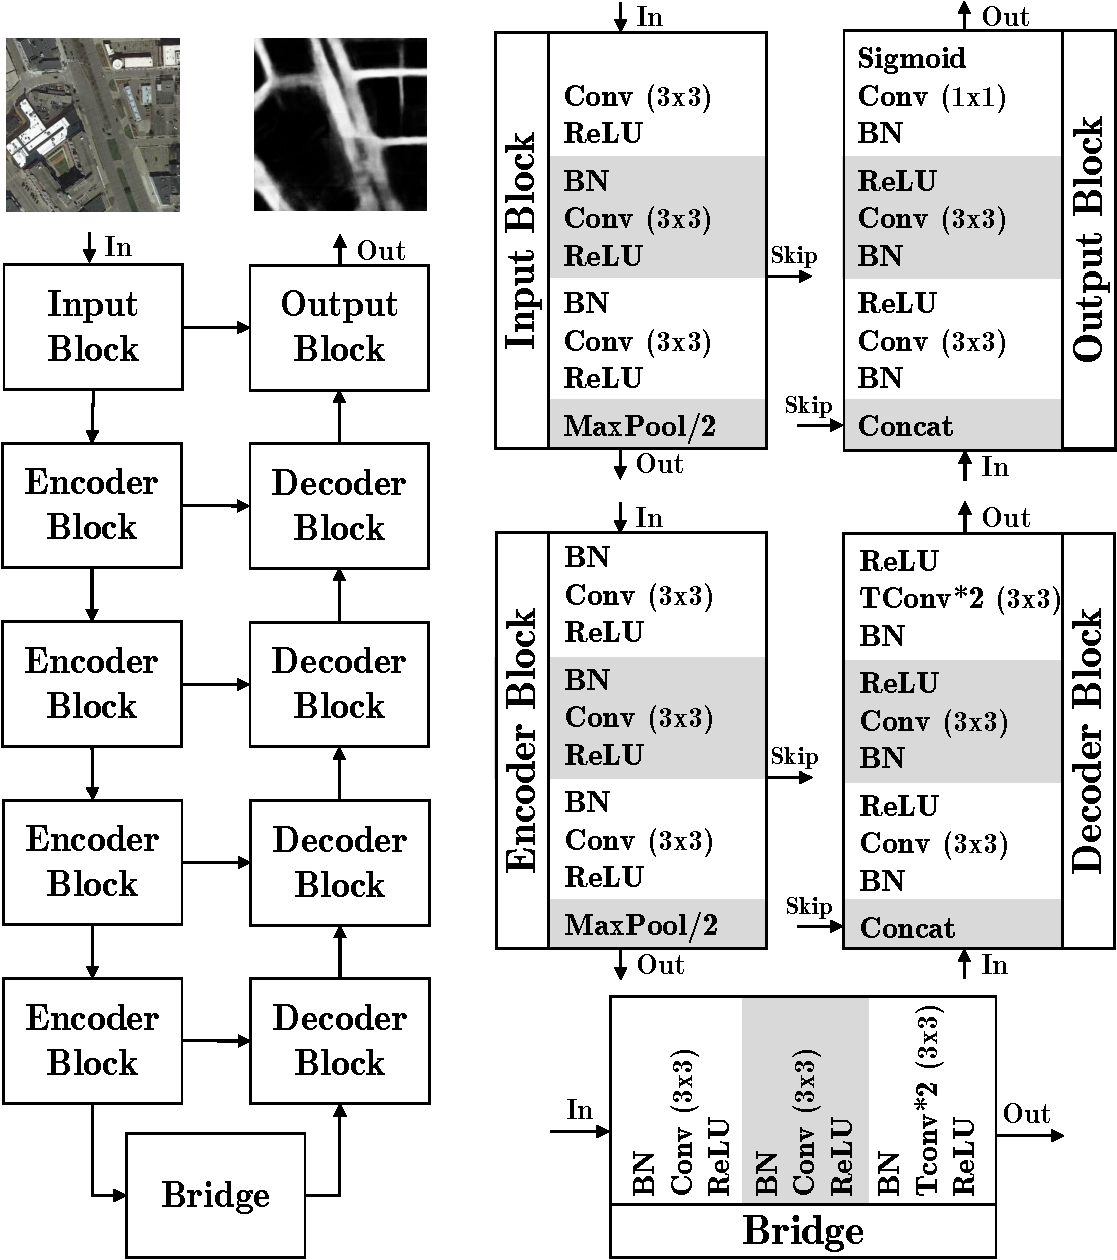
\includegraphics[width=0.85\columnwidth]{images/unet.pdf}
    \captionsetup{justification=centering}
    \caption{UNet - Architecture\\
    left: overall architecture, right: structure of each block}
    \label{fig:unet-arch}
\end{figure}
%\begin{figure}[ht]
%\centering
%    \begin{subfigure}
%        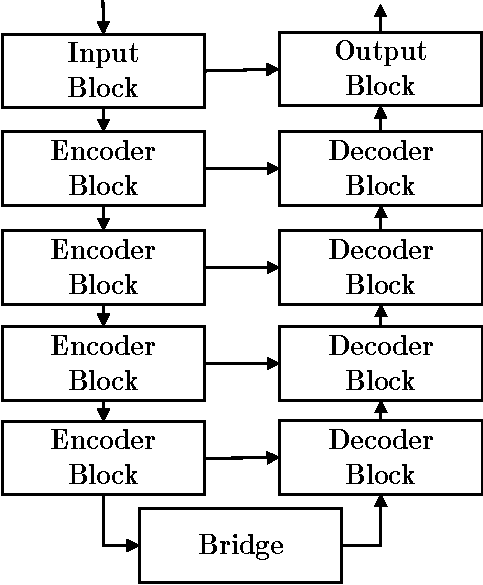
\includegraphics[width=0.55\columnwidth]{images/overview.pdf}
%    \end{subfigure}
%    \begin{subfigure}
%        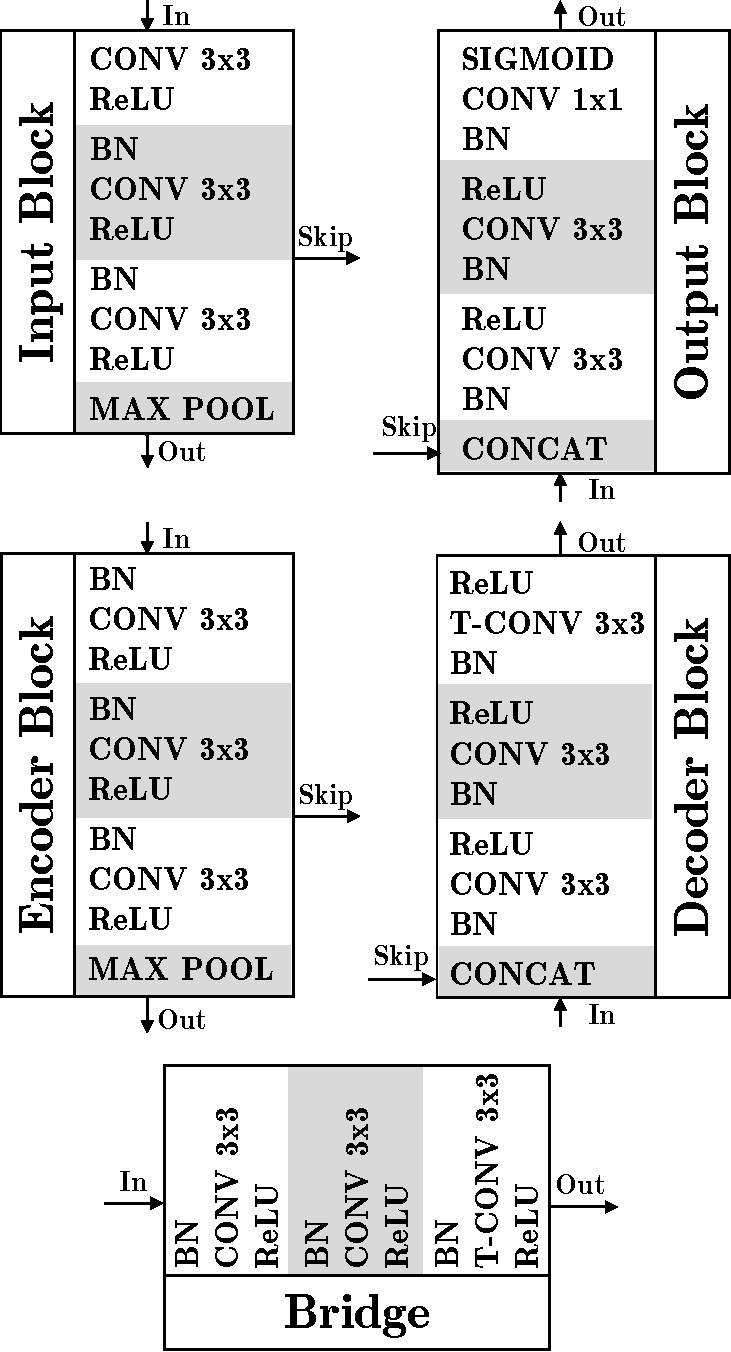
\includegraphics[width=0.35\columnwidth]{images/detail.pdf}
%     \end{subfigure}
%     \caption{UNet - Architecture}
%\end{figure}

The decoder, analogously to the encoder, consists of consecutive decoder blocks, each of which first concatenates the skip connection with the input from the previous level, before three runs of a sequence of again batch normalization, 3x3 convolution and ReLU. With the exception of the last repetition which uses a 3x3 transpose convolution with stride 2 to reverse the halving of the width and height during the encoding (see \textit{figure~\ref{fig:unet-arch}}). Throughout the network 64 filters are used except for the convolution right after the concatenation layers which uses 96 filters.

For the training we have used a patch-based approach to decrease uncertainty by extracting random patches of size 256x256 of a training image.

We have trained the UNet in 75 epochs, with a batch-size of 4 and 100 batches inside each epoch. The UNet uses an exponential learning rate, which we initially set to 0.005 with a decay of 0.95 and 1000 decay steps. For the validation we have used the same patch-size with stride 72.\\

\subsubsection{SqueezeNet}
Since the SqueezeNet was not originally designed for image segmentation we had to adjust its architecture from~\cite{CoRR1} to fit the needs of the task at hand. We used the original design (with the exclusion of the last two layers) to construct an encoder to bring the data to a smaller latent space. For the decoder we took the same structure but inversed it (see \textit{figure~\ref{fig:squeeze-arch}}). This made it possible to retrieve a black and white image consisting of the prediction probabilities for each pixel (see \textit{section~\ref{sec:predictions}} for details on the output format). Inspired by the architecture of the UNet, we added skip connections between each layer implemented as additions of the outputs of one side to the other.

\begin{figure}[ht]
\centering
     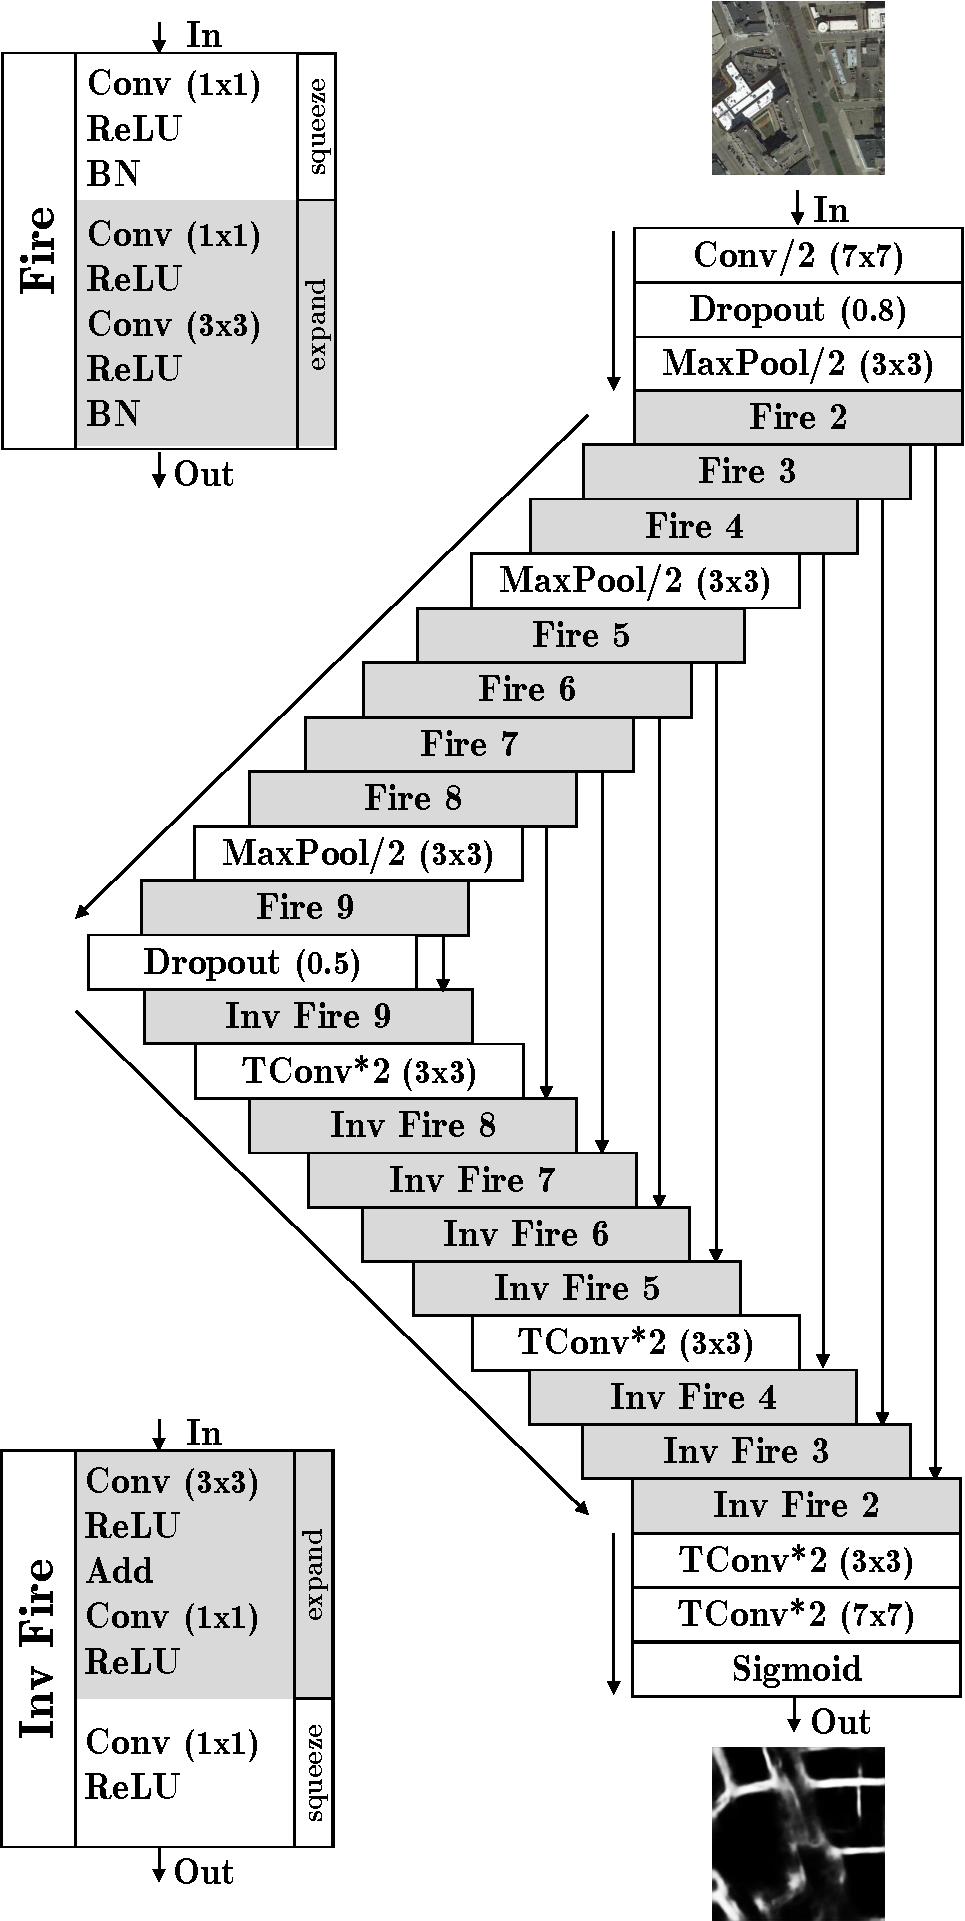
\includegraphics[width=0.75\columnwidth]{images/squeeze.pdf}
     \captionsetup{justification=centering}
     \caption{SqueezeNet - Architecture}
     \label{fig:squeeze-arch}
\end{figure}

The main blocks in this model are called \textit{fire modules}. Each fire module consists of a \textit{squeeze} and \textit{expand} part. We distinguish between a regular fire module and an inverse fire module, which appear in the decoder part and perform the squeeze and expand in reversed order. The squeeze part consists of a 1x1 convolution filter, ReLU and batch normalization, with the expand part consisting of a 1x1 convolution filter and ReLU, followed by a 3x3 convolution filter another ReLU and batch normalization. The inverse fire module follows a similar structure (see \textit{figure~\ref{fig:squeeze-arch}} for the structure of the respective modules).

The number of filters and the sizes correspond to the ones used in~\cite{CoRR1}. We have used a total of 8 fire modules. For the first two fire modules we begin with 16 filters for the squeeze component and 64 for the expand component. The number of filters used in the squeeze and expand modules increases by 16 and 64 every 2 fire modules. It is important to note that the same sizes are used for the inverse fire modules and correspond to the same numeration as in the fire modules.

As a further step for regularization and to increase the precision we included a \textit{dropout layer}, which drops a channel from a pixel with a probability of 20\%. This way the model is able to generalize better as parts of the image are not available.

The model was trained for 45 epochs, with 100 batches per epoch and a batch-size of 32. The used learning rate was 0.0001 and it was fixed for the entirety of the training process. As opposed to our patch-based approach for the UNet, we used the whole image for both training and validation.

\subsection{Making Predictions}
\label{sec:predictions}
The output of both models are matrices of per pixel prediction probabilities, visualized as black and white images with white representing a road prediction of probability 1 and black probability 0 (i.e. $p_{road} = pixel encoding/255$).

For the UNet we have additionally applied an \textit{ensemble} approach, i.e. we averaged over (0$^{\circ}$, 90$^{\circ}$, 180$^{\circ}$, 270$^{\circ}$) rotations with patch sizes 256x256 with stride 88 and the full image size 608x808.

From these per pixel predictions we have arrived at the 16x16 patch-wide prediction by calculating the mean of each patch and applying a 0.25 probability threshold to classify a patch as a road.

\subsection{Post-processing using CRF and averaging}
For the post-processing with CRF we used the inference algorithm described in~\cite{NIPS2011_4296} and provided by the library \textit{pydensecrf} from~\cite{PydenseGL}, which enables efficient inference on a pixel basis as opposed to a region basis and could therefore easily be embedded in our overall architecture.

We used the prediction probabilities output by the models as the unary potential. For our results we ran the algorithm for 25 inference steps. We were able to obtain the best results by keeping the strength of the pair-wise Gaussian location potentials low. This would normally make the segmentation less smooth, but worked to our advantage in this case, since smoothness with regards to location only would remove many correct road predictions. The opposite was the case with regards to the bilateral potentials taking colors into account: by raising their strengths we were able to create smoother clusters of predictions based on colors, i.e. a stray prediction of a road on a background of a different color (e.g. a nearby grass patch) would be removed. 

It is important to note that the CRF post-processing results in a strict \{0,1\} per-pixel prediction matrix.

The averaging function we have implemented is a simple per pixel average of the probability of two prediction probability matrices. We have again applied the 0.25 probability threshold to classify a patch as a road.

In the case of averaging after the CRF post-processing (as has been done for our final result), it should be noted that the \{0,1\} prediction output of the CRF means that the average results in a true overlay of the two solutions. 

\textit{Figure~\ref{fig:pred-pipeline}} shows a visualization of the full computational pipeline used to arrive at the final prediction mask.

\begin{figure}[ht]
\centering
    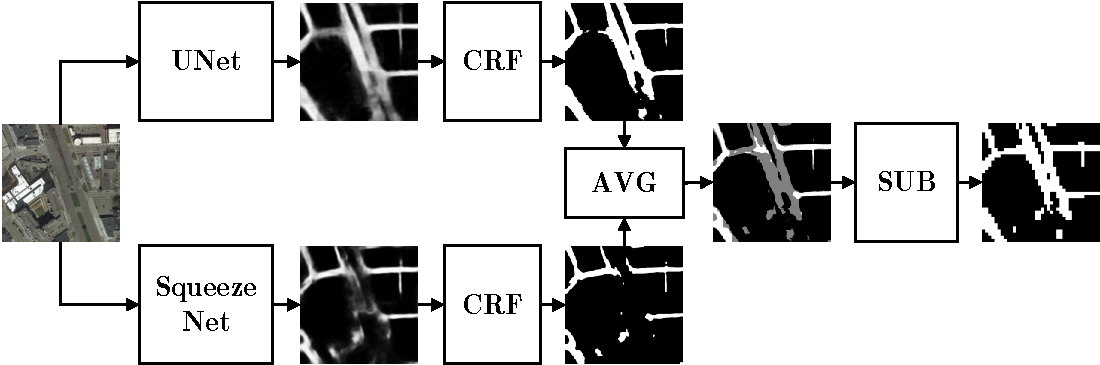
\includegraphics[width=\columnwidth]{images/best_result.pdf}
    \captionsetup{justification=centering}
    \caption{Full computation pipeline}
    \label{fig:pred-pipeline}
\end{figure}

\subsection{Dataset Extension}
\label{sec:dataset-extension}
During several test runs of our models, we have noted that the dataset provided for the training only represents part of the test images well. Many images in the test set raise challenges which have no counterpart in the training set. Difficulties we have observed were slim roads, or roads obscured by trees and/or shadows of buildings, large groups of cars, concrete which has been patched together and has different texture. For some cases, i.e. when the image is of a green area, there were no corresponding training samples at all.

The data augmentation we applied was only able to partially erase these difficulties. To achieve more accurate predictions, we therefore decided to extend the training set with manually labeled satellite images which we obtained from \textit{Google Earth} of the city of Berlin. We have chosen 46 images according to the challenges described above.

With this extension we were indeed able to get better results. In order to compare the different results easily we have added the choice of dataset (\textit{default}: originally provided training set, \textit{ext-half}: the original training set with half of the extended images, \textit{ext-full}: the fully extended training set) as a parameter to the model training. The extended data sets can be found in the repository~\cite{GitRepo}.

\section{Results}
All computations have been done on the \textit{Leonhard cluster} provided by ETHZ. (In order to reproduce the results the instructions in the readme file should be followed which can be found in~\cite{GitRepo} or the supplementary files.)\\
\begin{table*}[ht]
\centering
\begin{tabular}[c]{|l|l|l|l|}
  \hline
  Model&Training data set&Public score&Private score\\
  \hline
  Baseline 1 (linear regression)&default&0.39985&0.39115\\
  Baseline 2 (simple conv and maxPool layers)&default&0.86640&0.85138\\
  UNet (without CRF)&ext-full&0.87090&0.86028\\
  SqueezeNet (without CRF)&ext-half&0.88373&0.87360\\
  UNet (with CRF)&ext-full&0.89457&0.88433\\
  SqueezeNet (with CRF)&ext-half&0.88809&0.87808\\
  Prediction average of both models without CRF&(\textit{mixed})&0.88710&0.87912\\
  Prediction average of both models with CRF&(\textit{mixed})&0.89931&0.89082\\
  \hline
\end{tabular}
\captionsetup{justification=centering}
\caption{
  Private and public scores obtained on \textit{Kaggle} showing the  outputs\\
  produced by the various models and processing parameters.
}
\label{tab:scores}
\end{table*}
The results are given in \textit{Table~\ref{tab:scores}} in terms of the public and private scores assigned on the Kaggle competition site~\cite{KaggleComp}. While for our final and best result we used the process as described in \textit{figure~\ref{fig:pred-pipeline}}, we have also added the scores of each individual step. For comparison two baseline solutions have also been added.

The first one uses the linear regression model with the pre-processing steps used in exercise 11 of the course. \\
The second baseline is a simple architecture using only convolution and max-pooling layers. It starts with two convolution layers with 32 and 64 channels correspondingly followed by a max-pooling layer. After that two blocks of convolution and max-pooling layer are applied. For the decoder part we use a convolution with 256 channels, 3 up-sampling layers which are refined by two convolution layers and a sigmoid activation.

Both baselines were trained using the default dataset provided for this project.

\section{Discussion}
What becomes clear from \textit{table~\ref{tab:scores}} is that all of our models, either individually or in combination, scored higher than the two baselines.

For both the UNet and the SqueezeNet predictions the CRF post-processing was shown to improve the prediction accuracy. Especially the scores of the UNet improved. This is due to the fact that the UNet has made many more false road classifications as the SqueezeNet, which shows the effectiveness of the CRF in this regard.  \textit{Figure~\ref{fig:crf-comp}} shows an example of the results of successful CRF post-processing on an image with many false predictions.  While the CRF post-processing also removed some correct predictions, these were outweighed by the number of desired removals.

\begin{figure}[ht]
  \centering
  \captionsetup{justification=centering}
  \begin{subfigure}{.4\columnwidth}
    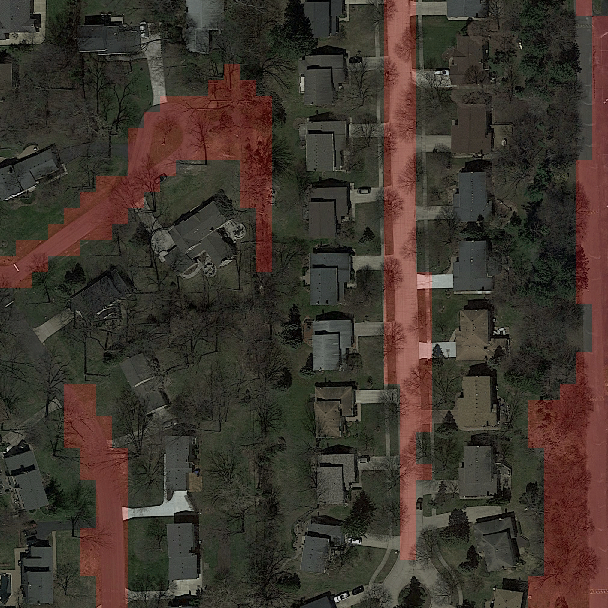
\includegraphics[width=\linewidth]{images/test_7_unet_beforepp.png}
  \end{subfigure}
  \begin{subfigure}{.4\columnwidth}
    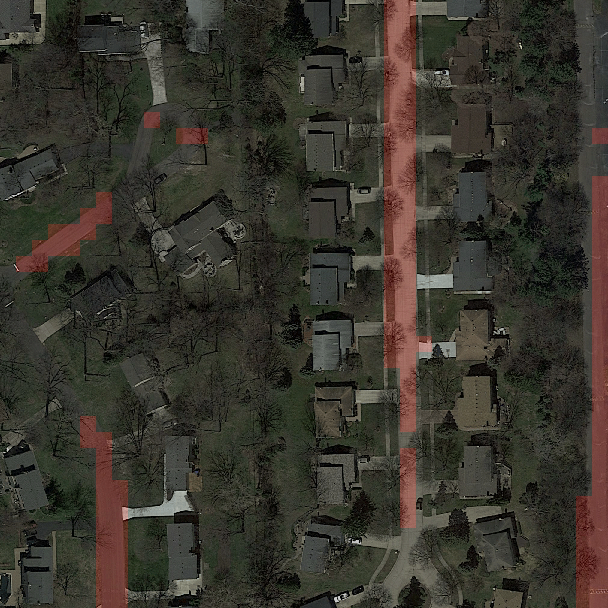
\includegraphics[width=\linewidth]{images/test_7_unet_afterpp.png}
  \end{subfigure}
  \caption{Road predictions for \textit{test\_7.png} from UNet before (left) and after (right) post-processing with CRF}
  \label{fig:crf-comp}
\end{figure}

The UNet and SqueezeNet on their own were indeed able to predict different image areas. For many images the differences were quite significant as can be seen in \textit{figure~\ref{fig:comp}}. As hoped by combining the two solutions of the UNet and the SqueezeNet we were able to obtain better results. However, without the CRF post-processing the improvements were not as prominent.
%This can be explained by the fact that while pixel-wise averaging is %already somewhat effective in removing false road classifications %(although nowhere near as CRF), on other occasions it could potentially %increase it.

\begin{figure}[ht]
  \centering
  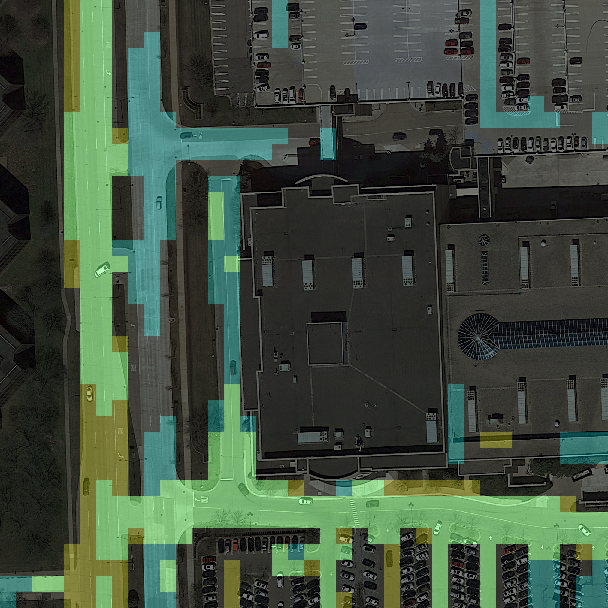
\includegraphics[width=0.5\columnwidth]{images/comp_10.png}
  \captionsetup{justification=centering}
  \caption{Comparison of the UNet (yellow) and SqueezeNet (blue) road predictions for \textit{test\_10.png} (green: both predicted a road)}
  \label{fig:comp}
\end{figure}

We could potentially have obtained even better results by combining more than two models. The choice of the prediction probability threshold also has proven to be quite tricky and further adjustments might also have an effect. Additionally, a modification in the post-processing pipeline order together with threshold adjustments could also increase the prediction accuracy.

Additionally it should be noted that we had initially trained the SqueezeNet model on the \textit{ext-half} data set and for time reasons were not able to run it again on the \textit{ext-full} as we had done for the UNet model. Doing this could have potentially yielded even better results.

\section{Summary}
As shown in our results, by combining the three separate techniques, the UNet model, SqueezeNet model and CRF post-processing, we were able to take advantage of their respective strengths and obtain better results than each on their own.

We were also able to design an adaptation of the SqueezeNet architecture for image segmentation.

\bibliographystyle{IEEEtran}
\bibliography{biblio}

\end{document}
